% LEAP: A Space Mission Design Game -- project description for NASA Space Apps 2026.
% Build: pdflatex leap-project-description.tex (twice, for the table of contents).
\documentclass[11pt,a4paper]{article}

\usepackage[T1]{fontenc}
\usepackage[utf8]{inputenc}
\usepackage{lmodern}
\usepackage{textcomp}
\usepackage[margin=2.2cm]{geometry}
\usepackage{graphicx}
\usepackage{booktabs}
\usepackage{tabularx}
\usepackage{array}
\usepackage{enumitem}
\usepackage[table]{xcolor}
\usepackage{caption}
\usepackage{float}
\usepackage[hidelinks]{hyperref}
\usepackage{xurl}

\definecolor{leapblue}{HTML}{1F4E8C}
\hypersetup{colorlinks=true, linkcolor=leapblue, urlcolor=leapblue, citecolor=leapblue}
\setlist{itemsep=2pt, topsep=4pt}
\newcolumntype{L}{>{\raggedright\arraybackslash}X}
\renewcommand{\arraystretch}{1.25}
\graphicspath{{figures/}}

\title{\textbf{LEAP: A Space Mission Design Game}\\[4pt]
  \large Launch \textperiodcentered{} Engineer \textperiodcentered{} Advance \textperiodcentered{} Pioneer\\[10pt]
  \normalsize NASA Space Apps Challenge 2026 \textperiodcentered{} Challenge: \emph{Space Mission Design Game}}
\author{Team Artemis IV}
\date{15 November 2026}

\begin{document}
\maketitle



\tableofcontents
\bigskip

% ---------------------------------------------------------------------------------------------------------------
\section{Team details}

\begin{table}[H]
\centering
\begin{tabularx}{\textwidth}{@{}l L L@{}}
\toprule
\textbf{Member} & \textbf{Programme} & \textbf{University} \\
\midrule
Tarek Bshinnati & Electrical and Computer Engineering, 4th year & American University of Beirut (AUB) \\
Mohammed Daouk & Electrical and Computer Engineering, 4th year & American University of Beirut (AUB) \\
Moataz Maarouf & Electrical and Computer Engineering, 4th year & American University of Beirut (AUB) \\
Muhammad Alaa Al Deen Al Hamwi & Computer Science, 2nd year & American University of Beirut (AUB) \\
\bottomrule
\end{tabularx}
\caption*{Team name: \textbf{Artemis IV}. Location: Beirut, Lebanon.}
\end{table}

% ---------------------------------------------------------------------------------------------------------------
\section{Problem statement}

There currently are no fun and accurate (historically and scientifically) space mission design games that help
children and adults learn about the history and design of space missions.

% ---------------------------------------------------------------------------------------------------------------
\section{Our solution}

Our solution is a game called \textbf{LEAP: A Space Mission Design Game} (LEAP stands for Launch, Engineer, Advance,
Pioneer). It is a 2.5D tycoon game: you run a small space company, build up its economy, and then design, launch and
fly real-style space missions. The goal is to make the trade-offs in the challenge brief (mass, power, budget, data,
communications, time) something players feel, not just read about. The game is a fun and educational experience,
meant to teach children and adults alike about the history of NASA and space missions, while letting them learn the
basics of space mission design in a fun and interactive way.



\paragraph{Tycoon economy.} Players build mines, factories and other buildings to produce spacecraft parts, then
upgrade them over time. The economy feeds the missions but never blocks them, since parts can also be bought.

\paragraph{Mission design.} Players take a contract, design a spacecraft from parts (bus, power, battery,
communications, pointing, propulsion and instruments), pick a launch vehicle and launch site, check the weather and
launch window, run a free test simulation, and then launch.

\subsection{Mission gameplay}
\begin{itemize}
  \item Every choice shows its effect live on the six resources from the brief.
  \item A test run estimates the chance of success before money is spent on a real launch.
  \item During flight, problems (``anomalies'') show up as short mini-games, such as pointing the antenna, freeing a
        stuck solar panel or surviving an eclipse on battery. They are more likely when the design has weak margins.
  \item After each mission, a report explains \emph{why} it worked or failed, not just whether it did, grouped under
        NASA's four mission segments (user, space, ground and launch).
  \item Optional launch insurance adds a simple risk decision.
\end{itemize}

\subsection{History campaign}
In the main mode the player starts in 1958 as a fictional contractor in the United States and works through real
milestones: Explorer~1, TIROS-1, Telstar~1, Syncom~3, Apollo~11, and the Artemis era with Artemis~II, III and IV.
Each milestone has a short ``Real History'' card with what actually happened and a link to learn more. Failures are
part of it too, such as Vanguard TV3 in 1957. Technology and rockets unlock era by era, matching what really existed
at the time. In the Artemis era the player chooses how the company helps Artemis~III and IV (for example a camera
satellite, a lunar relay, a cargo lander on the south-pole ridge or a Moon mapper), following NASA's published plans.

\subsection{Starting location and launch weather}
The starting location matters. Players pick a spot on a globe or roll a random seed, and the game uses real NASA
POWER climate data (sunshine, wind, rain and temperature) to shape the map and the launch weather. Latitude and
being near the coast affect launches, as they do for real spaceports: a launch can be scrubbed by wind or storms, and
Earth's spin at the launch site changes what a rocket can lift.

\subsection{Launch progression}
In the early eras, players build spacecraft and pay to launch them on the rockets of the time, the way AT\&T paid
NASA to launch Telstar. Saturn~V, the Space Launch System and modern rideshares follow in later eras.

\subsection{Free Play mode}
Besides the campaign, a Free Play mode offers generated contracts. Each says who needs the data (a farmer, a
fishing crew, a mountain village), and the player can also start from a question, such as ``Where are storms
forming?'', which sets the orbit, instrument and mission length.

\subsection{Audience and online safety}
The audience includes students and people of all backgrounds from about age 10. The online features are kept safe:
no chat, anonymous accounts with a generated nickname, no personal data, and only preset actions between players.
Two game modes, described next, let children enjoy a simple, educational experience while adults can take on a
harder game with more technical detail.

\subsection{Two modes: Explorer and Mission Director}
Both modes play the same missions under the same rules; the player picks one when starting a company.
\begin{itemize}
  \item \textbf{Explorer} (beginner, from about age 10): bars with icons and plain words instead of numbers and
        units; a ``ghost'' preview on the resource bars that shows how each part would change them before it is
        chosen; a shorter, four-step Launch planner (rocket, launch site, weather, launch) with a tick-and-cross
        checklist; a simple mission report that leads with the result and lists what went right and wrong; bigger,
        colour-blind-safe controls; NASA pages for young readers as ``learn more'' links; gentler failure (one refund
        per contract) and shorter waits.
  \item \textbf{Mission Director} (advanced): every number and unit, every part and all seven planning steps, the
        mission report grouped under NASA's four segments with the design's own numbers, design margins in the style
        of JPL's concept maturity checklist, contract offers that expire, paid repeat test runs, costlier ground tests,
        mineral deposits that run out, and NASA papers and slides as reading.
\end{itemize}
An Explorer company can move up to Mission Director at any time, keeping its progress. How the split follows research
on learning from space games is in Section~\ref{sec:learning}.

\subsection{Minigames mode}
A separate mode from the main menu offers short 2D games for each level. The player picks Explorer or Mission
Director and plays that level's three games in a random order. Each game ends on one real space fact (in plain
words in Explorer), a star score and a link to read more: a NASA Space Place page in Explorer, a NASA page in Mission
Director. These Minigames are separate from the anomaly mini-games that happen during a mission.

\begin{table}[H]
\centering\small
\begin{tabularx}{\textwidth}{@{}l p{3.3cm} L L@{}}
\toprule
\textbf{Level} & \textbf{Game} & \textbf{What the player does} & \textbf{The fact it teaches} \\
\midrule
Explorer & Build Pluto & Catch rock for the core and ice for the shell, and dodge the gas. & Pluto became a dwarf planet in 2006; it is rock and ice, not gas \cite{pluto, spaceplace}. \\
Explorer & Rover Rescue & Drive a rover to glowing rocks, drill samples and bring them to the lab before the battery runs low. & Mars rovers drive, drill and study rock samples \cite{perseverance, curiosity}. \\
Explorer & Planet Parade & Put the planets in order from the Sun, then by size. & The planets' order and their real sizes \cite{planetfacts}. \\
Mission Director & Too Hot, Too Cold & Keep four parts of a small satellite in their temperature bands for four orbits, with heaters that cost power and three radiator louvers to share. & Every part has a temperature range; heaters and radiators keep it there \cite{thermal}. \\
Mission Director & Square Peg, Round Hole & Build an air path from the cabin fan through a square canister to Apollo~13's round socket, with bags, cardboard and tape. & Apollo~13's carbon dioxide fix in April 1970 \cite{apollo13}. \\
Mission Director & Lost Signal & Work the loss-of-signal checklist for a probe whose antenna points 2\textdegree{} off Earth, and wait out the light time. & Voyager~2's loss of contact in 2023, the Deep Space Network and how signals fade with distance \cite{voyager2, dsn}. \\
\bottomrule
\end{tabularx}
\end{table}
\noindent Status: all six games are built, in the game and played through at two screen sizes.

\subsection{Multiplayer and weekly challenges}
Players can create an anonymous account and compare scores on a leaderboard. They can also enter a weekly
challenge with the same budget and parts for everyone; the score favours reliability, then science value, then money
and mass left over. Speed does not count, so people can play on any day of the week.

\subsection{Technical implementation and visual style}
LEAP is a browser game (TypeScript, Vite and three.js, with Supabase for the online part), so it runs on Windows,
macOS, Linux and Chromebooks with no install. The look is realistic 3D with a clean, simple interface and short
text: textured terrain and sea, buildings, rockets and pads modelled in Blender, Earth from NASA imagery and the Moon
from NASA's lunar data. Anyone can play it on any desktop or laptop, which lets us reach as many people as possible.

\subsection{What is built (15 November 2026)}
\begin{itemize}
  \item Eras 1 and 2 (1958--1964), Era 3 (Apollo~11) and the Artemis era (Artemis~II, III and IV, the finale), plus
        Free Play and a Demo Mode that opens a ready company in one click.
  \item The Mission Designer with six live resource bars, the Launch planner under the four segments, ground tests,
        the free test run, 3D launches with staging, and Moon sequences for Apollo~11 and Artemis that the player can
        look around in.
  \item Two game modes on one rule set: Explorer for beginners and Mission Director for realism.
  \item Anomaly mini-games, the mission report, mission patches, the History Archive, Team Mode for up to four
        players on one screen, and the optional online features.
\end{itemize}

\begin{figure}[H]
\centering
\begin{minipage}{0.49\textwidth}\centering
  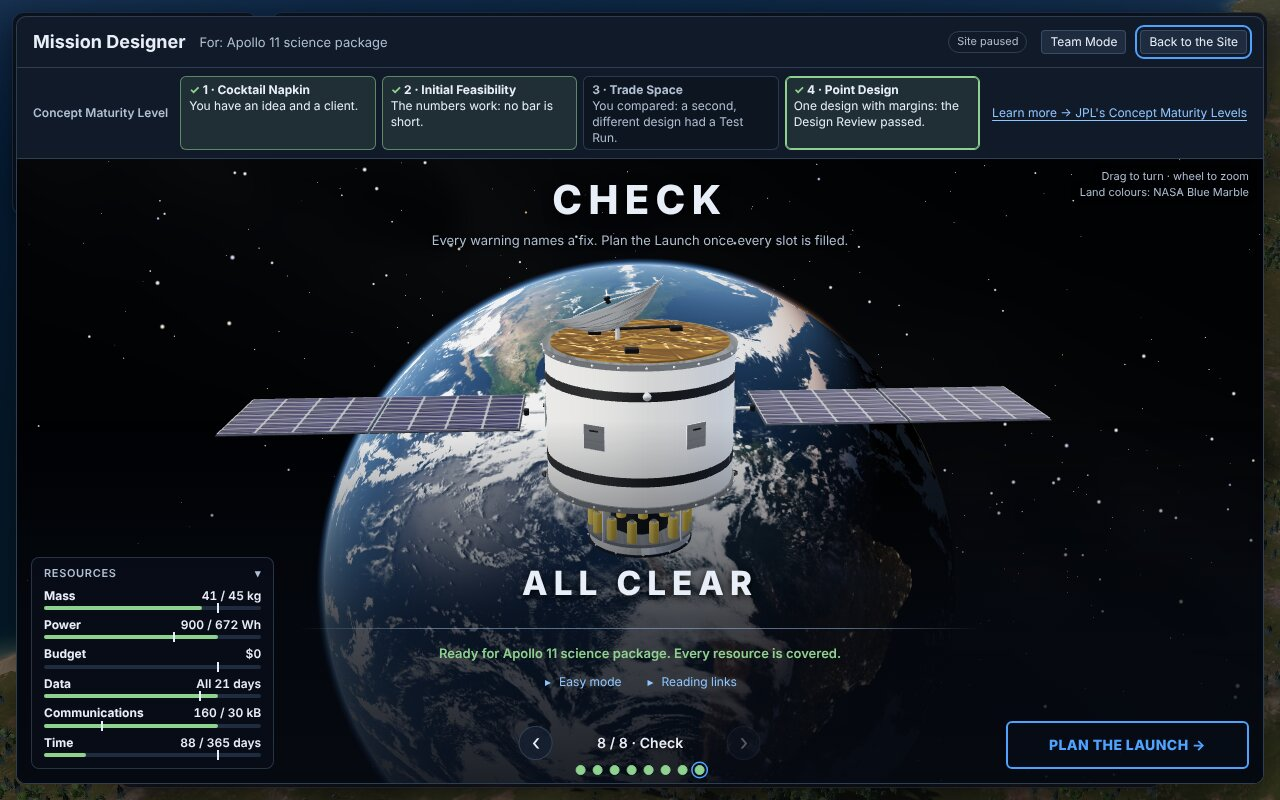
\includegraphics[width=\linewidth]{designer-apollo11.jpg}
  \captionof{figure}{Mission Designer: the Apollo~11 science package, with the six resources bottom left.}
\end{minipage}\hfill
\begin{minipage}{0.49\textwidth}\centering
  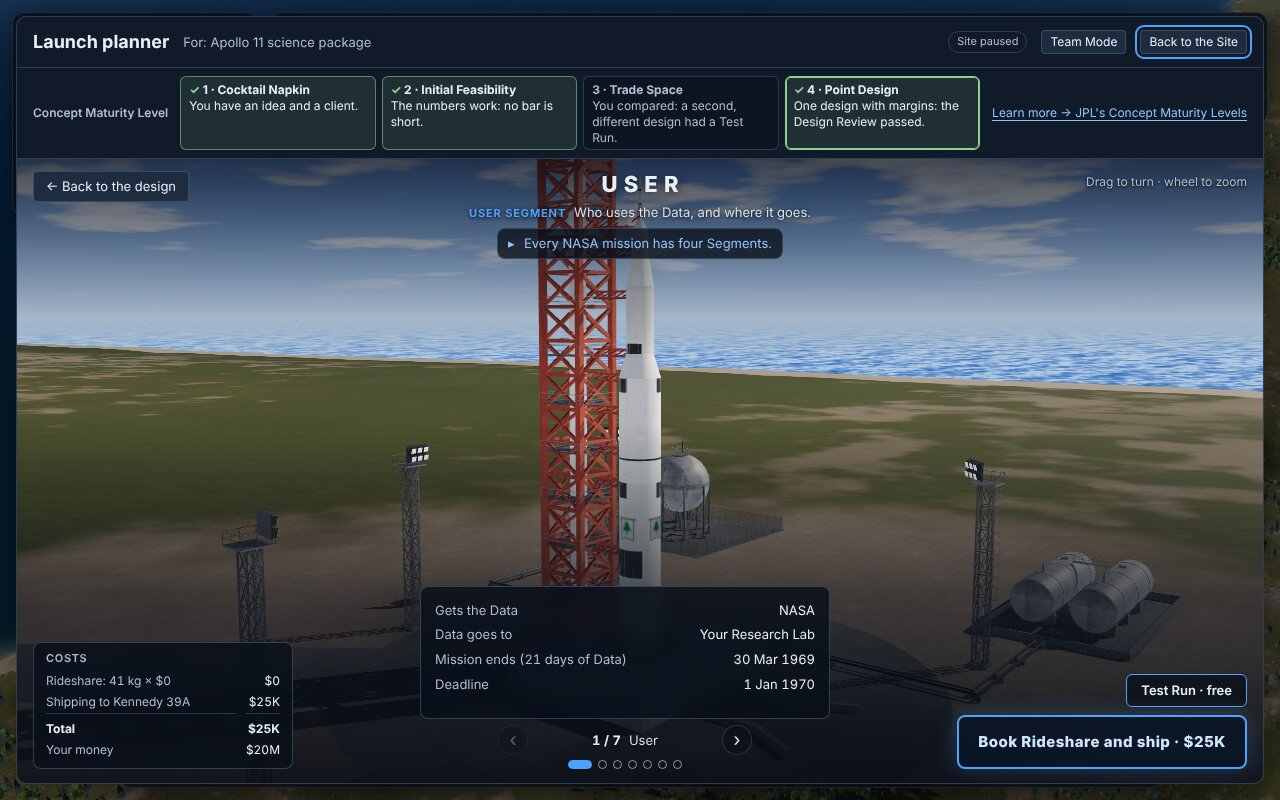
\includegraphics[width=\linewidth]{planner-saturn-v.jpg}
  \captionof{figure}{Launch planner: Saturn~V on Kennedy LC-39A, starting with the user segment.}
\end{minipage}

\vspace{8pt}
\begin{minipage}{0.32\textwidth}\centering
  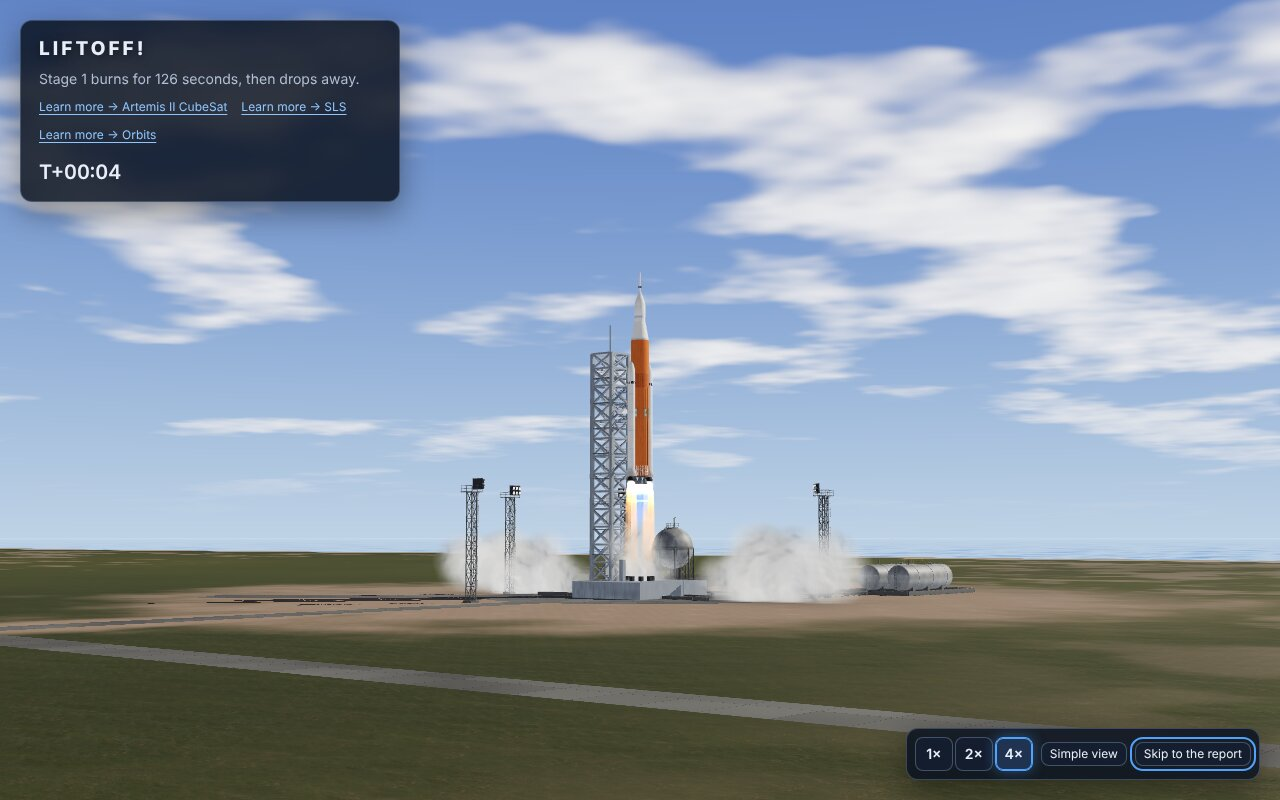
\includegraphics[width=\linewidth]{sls-liftoff.jpg}
  \captionof{figure}{SLS lifts off from LC-39B with the player's CubeSat (Artemis~II).}
\end{minipage}\hfill
\begin{minipage}{0.32\textwidth}\centering
  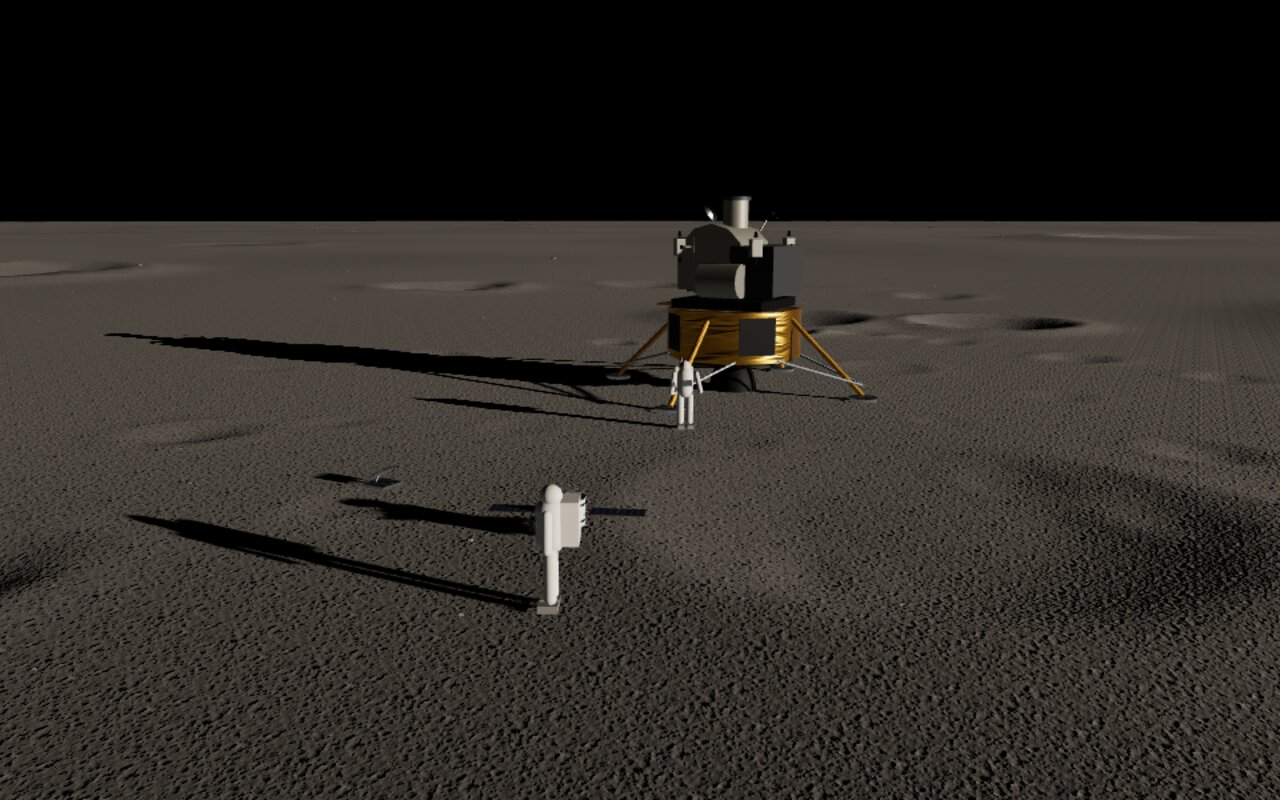
\includegraphics[width=\linewidth]{apollo11-surface.jpg}
  \captionof{figure}{Tranquility Base: the crew sets up the player's science package.}
\end{minipage}\hfill
\begin{minipage}{0.32\textwidth}\centering
  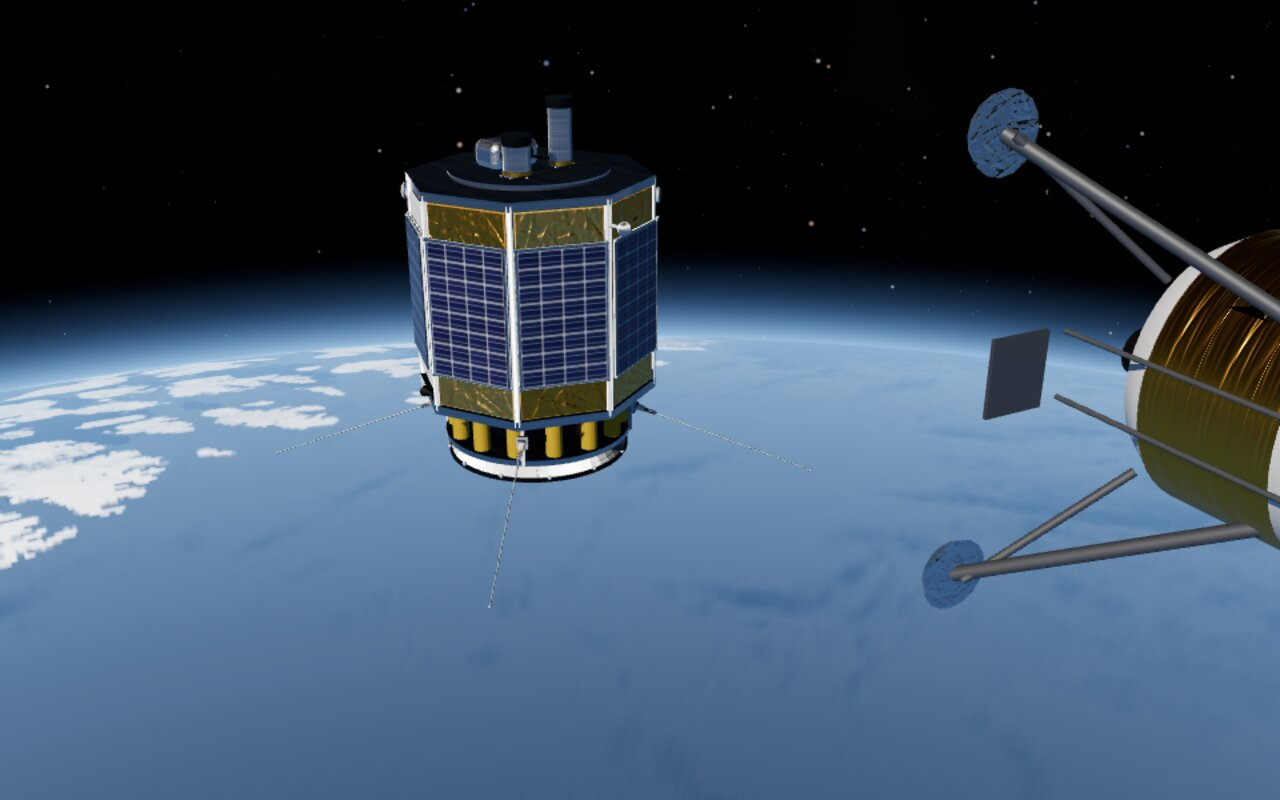
\includegraphics[width=\linewidth]{artemis3-satellite.jpg}
  \captionof{figure}{Artemis~III: the player's satellite near the lander test article, 440~km up.}
\end{minipage}
\end{figure}

% ---------------------------------------------------------------------------------------------------------------
\section{Research findings}

Every fact and number in LEAP is cited; the full notes, with a source for each claim, are in the repository's
\texttt{docs/research/} folder. The main findings that shaped the game:

\subsection{How NASA designs a mission}
\begin{itemize}
  \item NASA's \emph{Design and Develop Science Missions} (Small Spacecraft institute, 2025), one of the challenge's
        official resources, splits every mission into four segments: user, space, ground and launch. It describes six
        steps, from ``Identify Need \& Goals'' to ``Implement'', and advises to ``begin with the end in mind'': start
        from who uses the data \cite{segments}. LEAP's Launch planner and mission report follow the four segments, the
        tutorial follows the six steps, and every contract starts with who needs the data.
  \item JPL's Concept Maturity Levels run from CML~1 (``Cocktail Napkin'') to CML~9; at CML~4 (``Point Design'') the
        checklist asks for at least 35\% margin on dry mass, power and energy \cite{cml}. LEAP shows a maturity strip
        and passes a design review when the margins are met.
  \item NASA's \emph{CubeSat 101} explains how small satellites get rides and why designs should be kept simple
        \cite{cubesat101}; its pages are linked from the game's tips.
\end{itemize}

\subsection{Physics and launch sites}
\begin{itemize}
  \item Earth's surface at the equator moves east at about 465~m/s, so rockets launched east near the equator need
        less fuel or carry more \cite{spaceport}. At Cape Canaveral (28.4\textdegree{}~N) the ground moves at about
        409~m/s, at Wallops Island (37.8\textdegree{}~N) about 367~m/s. In the game, each site's ground speed changes
        a rocket's lift.
  \item NASA POWER's daily data give wind, rain and temperature at each launch site; the game scrubs a launch for
        wind over 12~m/s, and treats heavy rain on a hot day as a thunderstorm, after NASA's lightning launch rules
        \cite{power}.
  \item Orbits use real values for Earth's gravity, radius and rotation; the Space view shows reference paths computed
        with NASA's GMAT, taken from NASA Mission Viz \cite{missionviz, gmat}.
\end{itemize}

\subsection{Real spacecraft parts}
\begin{itemize}
  \item Modern multi-junction solar cells reach about 30\% efficiency (up to 34\%); fold-out arrays give about
        40--140~W/kg; lithium-ion cells store about 150--270~Wh/kg (NASA's \emph{State of the Art of Small Spacecraft
        Technology}) \cite{soa}. Early satellites used mercury batteries: Explorer~1 was powered only by them
        \cite{explorer1}.
  \item Part masses, power and data rates in the game are tuned within these real ranges, and each mission report
        compares the player's spacecraft with the real one it is modelled on.
\end{itemize}

\subsection{Learning from space games: why two modes}\label{sec:learning}
Two studies of educational space games shaped how LEAP splits Explorer from Mission Director.

\paragraph{Cao, Peng and Hansberger (2019)} built a serious game on the Apollo~16 lunar mission: players plan a rover
route on a lunar map, pick and load equipment, then drive while watching direction, speed and motor and battery
temperature. With 30 participants, a virtual-reality version raised interest in space science and lunar history more
than a standard-screen version, but was harder to operate and took longer; practice closed part of the gap. The study
measured usability, engagement and interest, not factual learning \cite{cao2019}.

\paragraph{Herder and Rau (2022)} studied students playing the astronomy game \emph{At Play in the Cosmos}, which uses
tools such as spectrum analysers and radial-velocity displays. A high-performing student could operate the tools
without understanding the science behind them. In an experiment (45 students, 43 analysed), players got better at
recognising patterns in the visuals but showed no significant gain in explaining what they meant or in astronomy
knowledge, and added instructional prompts did not help significantly. Using a game's interface is not the same as
understanding the science \cite{herder2022}.

\begin{table}[H]
\centering\small
\begin{tabularx}{\textwidth}{@{}p{4.2cm} L L@{}}
\toprule
\textbf{Finding} & \textbf{Explorer (beginner)} & \textbf{Mission Director (advanced)} \\
\midrule
Build learning into connected mission phases \cite{cao2019}. & Contract, design, launch plan, flight and report in order, with a four-step planner. & The same chain with all seven planning steps; each phase's numbers carry into the next. \\
Balance immersion with ease of use; let players practise first \cite{cao2019}. & Short texts, bigger controls, gentler failure and a refund, so a first failure is a lesson, not a wall. & The full detail once the player is ready; an Explorer company can move up and keep its progress. \\
Give meaningful scientific choices with authentic details \cite{cao2019}. & Real parts, rockets, launch sites and weather, shown in words and pictures. & Real numbers and units, cited facts, real launch weather and margins. \\
Design for accessibility and comfort \cite{cao2019}. & Colour-blind-safe, larger interface; plain mouse controls. & Full 3D views to look around in. Both modes can skip a launch to its report or switch to a simple 2D view. \\
Connect data to what it means \cite{herder2022}. & The ghost preview shows a part's effect on the bars before it is chosen. & Six live resource bars with exact values and margins. \\
Using the interface is not understanding; make interpretation part of progress \cite{herder2022}. & The report says in plain words \emph{why} the mission worked or failed. & The report explains each result with the design's own numbers; the design review asks for margins, not just a working design. \\
Check understanding, not only task completion; simple prompts were not enough \cite{herder2022}. & \multicolumn{2}{>{\raggedright\arraybackslash}p{\dimexpr\textwidth-4.2cm-4\tabcolsep\relax}}{Not yet measured in LEAP. Our classroom tests will ask players to explain a failure, not only to fix it (see Next steps).} \\
\bottomrule
\end{tabularx}
\end{table}

\subsection{Mission history}
\begin{table}[H]
\centering\small
\begin{tabularx}{\textwidth}{@{}l l L@{}}
\toprule
\textbf{Milestone} & \textbf{Date} & \textbf{Fact used in the game} \\
\midrule
Explorer 1 & 31 Jan 1958 & First US satellite, launched before NASA existed; its radiation detector found the Van Allen belts \cite{explorer1}. \\
TIROS-1 & 1 Apr 1960 & First full-scale weather satellite; worked 78 days \cite{tiros}. \\
Telstar 1 & 10 Jul 1962 & First privately funded space project: AT\&T paid NASA for the launch \cite{telstar}. \\
Syncom 3 & 19 Aug 1964 & First geostationary communications satellite; carried the 1964 Tokyo Olympics to the US \cite{syncom}. \\
Apollo 11 & 16--24 Jul 1969 & The crew left a seismometer and a laser reflector (77~kg together); scientists still bounce lasers off the reflector \cite{a11, sp4205}. \\
Artemis II & 1--10 Apr 2026 & First crewed flight around the Moon since 1972, on SLS from Kennedy LC-39B \cite{a2}. \\
Artemis III & planned 2027 & NASA's plan: Orion docks with lander test articles in low Earth orbit, about 440~km up \cite{a3}. \\
Artemis IV & planned 2028 & NASA's plan: the first crewed landing since 1972, near the lunar south pole \cite{a4}. \\
\bottomrule
\end{tabularx}
\end{table}

% ---------------------------------------------------------------------------------------------------------------
\section{NASA and partner-agency data}

\begin{table}[H]
\centering\small
\begin{tabularx}{\textwidth}{@{}p{3.6cm} L L@{}}
\toprule
\textbf{Data or resource} & \textbf{Provider} & \textbf{How LEAP uses it} \\
\midrule
NASA POWER & NASA Langley Research Center & Climate of every starting location (2025 monthly averages) and daily launch weather at Cape Canaveral and Wallops Island \cite{power}. \\
Blue Marble: Next Generation & NASA Earth Observatory, via NASA GIBS & Colours of the land on the 3D Earth \cite{bluemarble, gibs}. \\
Black Marble and VIIRS true colour & NASA Earth Observatory; NASA and NOAA, via NASA GIBS & City lights on Earth's night side; real clouds of one day \cite{blackmarble, viirs}. \\
CGI Moon Kit (LROC colour, LOLA elevation) & NASA Scientific Visualization Studio & The 3D Moon in the Moon sequences and the Space view \cite{moonkit}. \\
NASA Image and Video Library & NASA & Photos on the Real History cards, each credited \cite{nasaimages}. \\
Design and Develop Science Missions & NASA Small Spacecraft institute & The four mission segments and six steps \cite{segments}. \\
Concept Maturity Levels & NASA JPL & The maturity strip and design review margins \cite{cml}. \\
NASA Mission Viz (GMAT trajectories) & NASA & Reference paths in the Space view \cite{missionviz}. \\
CubeSat 101 & NASA CubeSat Launch Initiative & Tips and reading links \cite{cubesat101}. \\
NASA history and science pages & NASA, NSSDCA, JPL, ALSJ & Facts on every Real History card and Moon sequence caption \cite{a11, sp4205, sp4029}. \\
Alouette 1 & Canadian Space Agency (partner agency) & A Real History card on Canada's first satellite (1962), which studied the ionosphere \cite{alouette}. \\
\bottomrule
\end{tabularx}
\end{table}

% ---------------------------------------------------------------------------------------------------------------
\section{Business opportunity and potential impact}

\subsection{Potential impact}
\begin{itemize}
  \item \textbf{Learning by doing.} Mission trade-offs usually stay abstract for students. In LEAP a player sees why a
        heavier battery needs a bigger rocket, or why the data did not fit through the antenna, and can fail safely and
        try again. The aim is a game a class can play in one lesson and still talk about the next day.
  \item \textbf{Reach.} LEAP runs in any modern browser, with no install, on school computers and Chromebooks. It is
        easy to start from about age 10, with depth for adults.
  \item \textbf{Trust.} Every number has a reason the player can read, every real mission links to its NASA source,
        and the game is built for children's safety (no chat, no personal data, anonymous accounts).
  \item \textbf{Space history for everyone.} The campaign tells the story from Explorer~1 to Artemis, including
        failures and partner-agency missions, so players see how space missions are really built.
\end{itemize}

\subsection{Path 1: adoption by NASA or another space agency}
Space agencies run education and outreach programmes and publish games and activities for students. LEAP is built
on NASA's own mission design material and data, so a natural path is for an agency's education or outreach office to
adopt it and take it to a deployment-ready version. That version would add:
\begin{itemize}
  \item classroom pilots with teachers, a teacher's guide, and lesson plans matched to school curricula;
  \item more eras and missions (Landsat, Hubble, the Lunar Reconnaissance Orbiter), agency-specific campaigns, and
        partner-agency milestones;
  \item translations (for example Arabic and French for our region), accessibility work and a review of every fact by
        agency subject experts;
  \item a security and privacy review of the online features, and hosting that scales to many schools.
\end{itemize}
The same model fits other agencies (for example ESA, the Canadian Space Agency, or the space agencies of the Arab
region), each with its own milestones and data.

\subsection{Path 2: independent release}
Without agency adoption, LEAP can still reach players and pay for its development:
\begin{itemize}
  \item a free browser version for individual players, with paid site licences for schools (classroom management,
        progress reports, teacher tools);
  \item a premium desktop release on game stores, with the full campaign and Free Play;
  \item custom mission packs and kiosk versions for science museums and planetariums;
  \item workshops and competitions built on the weekly challenge.
\end{itemize}


\subsection{Next steps}
\begin{enumerate}
  \item Make the repository public and host the game on GitHub Pages.
  \item Test both modes with students and teachers; measure what they learn before and after a lesson, including
        whether they can explain why a mission failed, not only fix it \cite{herder2022}.
  \item Finish the remaining eras and the planned features (trade studies, end-of-mission choices, more anomalies).
  \item Approach agency education offices and science museums with the classroom results.
\end{enumerate}

% ---------------------------------------------------------------------------------------------------------------
\section{Supporting documents}

All documents are in the project repository: \url{https://github.com/valgyrie/NASA-Space-Mission-Design-Game}.
The hosted game will be at \url{https://valgyrie.github.io/NASA-Space-Mission-Design-Game/}.

\begin{table}[H]
\centering\small
\begin{tabularx}{\textwidth}{@{}l L@{}}
\toprule
\textbf{Document} & \textbf{Contents} \\
\midrule
\texttt{docs/GDD.md} & Game design document: what the game is and every design decision. \\
\texttt{docs/research/} & Cited research notes: milestones, rockets, spacecraft parts, orbits, launch sites, weather, Eras 3--5. \\
\texttt{docs/research/learning-from-games.md} & Summaries of the two learning studies and how they map onto Explorer and Mission Director. \\
\texttt{docs/challenge.md} & The official challenge brief and resources. \\
\texttt{docs/adr/} & Architecture decision records (lasting technical choices and why). \\
\texttt{docs/tickets/} & The 53 feature tickets, each with what was built and how it was tested. \\
\texttt{docs/art/}, \texttt{docs/audio/} & Every 3D model, texture and sound with its author, source and licence. \\
\texttt{docs/eras-demo/notes-playtest.md} & Play-test notes for the Moon and Artemis eras. \\
\texttt{GLOSSARY.md}, \texttt{CHECKLIST.md} & Game vocabulary; everything done and still to do. \\
\bottomrule
\end{tabularx}
\end{table}

\paragraph{Tools and disclosure.} AI coding agents (Claude Code and Codex) wrote the code and the Blender model
scripts from the team's design documents and tickets; the team reviewed and tested every change. The music was
generated with Google Lyria and the era illustrations with image tools, each marked as AI-generated. The game idea
and design are the team's own, and facts and numbers come from cited sources, not from AI. Space Apps support
allowed our team to start before the hackathon; the git history shows every change and its date.

% ---------------------------------------------------------------------------------------------------------------
\begin{thebibliography}{99}\small

\bibitem{segments} J.~Levri, \emph{Design and Develop Science Missions}, NASA Small Spacecraft institute, 26 March 2025.
  \url{https://www.nasa.gov/wp-content/uploads/2025/04/250323-design-and-develop-science-mission.pdf}
\bibitem{cml} R.~Wessen, C.~Borden, J.~Ziemer, J.~Kwok, ``Space Mission Concept Development Using Concept Maturity Levels'', AIAA SPACE 2013, NASA JPL.
  \url{https://dataverse.jpl.nasa.gov/dataset.xhtml?persistentId=hdl:2014/44299}
\bibitem{cubesat101} NASA CubeSat Launch Initiative, \emph{CubeSat 101: Basic Concepts and Processes for First-Time CubeSat Developers}.
  \url{https://www3.nasa.gov/sites/default/files/atoms/files/nasa_csli_cubesat_101_508.pdf}
\bibitem{power} NASA Langley Research Center, NASA POWER (Prediction Of Worldwide Energy Resources). \url{https://power.larc.nasa.gov/}
\bibitem{bluemarble} NASA Earth Observatory (R.~St\"ockli), Blue Marble: Next Generation.
  \url{https://science.nasa.gov/earth/earth-observatory/blue-marble-next-generation/}
\bibitem{gibs} NASA Global Imagery Browse Services (GIBS). \url{https://nasa-gibs.github.io/gibs-api-docs/}
\bibitem{blackmarble} NASA Black Marble. \url{https://blackmarble.gsfc.nasa.gov/}
\bibitem{viirs} NASA Earthdata, VIIRS. \url{https://www.earthdata.nasa.gov/data/instruments/viirs}
\bibitem{moonkit} E.~Wright, CGI Moon Kit, NASA's Scientific Visualization Studio. \url{https://svs.gsfc.nasa.gov/4720}
\bibitem{nasaimages} NASA Image and Video Library. \url{https://images.nasa.gov/}
\bibitem{missionviz} D.~O'Neil, NASA Mission Viz. \url{https://nasa.github.io/mission-viz/}
\bibitem{gmat} NASA Goddard, General Mission Analysis Tool (GMAT), NASA Software Catalog GSC-19468-1.
  \url{https://software.nasa.gov/software/GSC-19468-1}
\bibitem{soa} NASA Small Spacecraft Systems Virtual Institute, \emph{State of the Art of Small Spacecraft Technology}, Power chapter.
  \url{https://www.nasa.gov/smallsat-institute/sst-soa/}
\bibitem{spaceport} Spaceport (on the equator's 465~m/s ground speed). \url{https://en.wikipedia.org/wiki/Spaceport}
\bibitem{explorer1} NASA History, ``60 years ago, Explorer 1 becomes America's first satellite''.
  \url{https://www.nasa.gov/history/60-years-ago-explorer-1-becomes-americas-first-satellite/}
\bibitem{tiros} NASA Science, TIROS. \url{https://science.nasa.gov/mission/tiros/}
\bibitem{telstar} NASA History, ``Telstar Opened Era of Global Satellite Television''.
  \url{https://www.nasa.gov/history/telstar-opened-era-of-global-satellite-television/}
\bibitem{syncom} NASA, ``The First Geosynchronous Satellite''. \url{https://www.nasa.gov/image-article/first-geosynchronous-satellite/}
\bibitem{a11} NASA, Apollo 11 Mission Report and Apollo Lunar Surface Journal. \url{https://www.nasa.gov/history/alsj/}
\bibitem{sp4205} C.~Brooks, J.~Grimwood, L.~Swenson, \emph{Chariots for Apollo}, NASA SP-4205 (NTRS 19790020032).
  \url{https://ntrs.nasa.gov/citations/19790020032}
\bibitem{sp4029} NASA SP-4029, \emph{Apollo by the Numbers}: Apollo 11 summary.
  \url{https://www.nasa.gov/wp-content/uploads/static/history/SP-4029/Apollo_11a_Summary.htm}
\bibitem{a2} NASA, Artemis II. \url{https://www.nasa.gov/mission/artemis-ii/}
\bibitem{a3} NASA, ``NASA's Artemis III mission to test future Moon lander operations'', 23 October 2026.
  \url{https://www.nasa.gov/missions/artemis/nasas-artemis-iii-mission-to-test-future-moon-lander-operations/}
\bibitem{a4} NASA, ``NASA, partners accelerate lander development for 2028 Moon missions'', 23 October 2026.
  \url{https://www.nasa.gov/missions/artemis/nasa-partners-accelerate-lander-development-for-2028-moon-missions/}
\bibitem{alouette} Canadian Space Agency, Alouette I and II. \url{https://www.asc-csa.gc.ca/eng/satellites/alouette.asp}
\bibitem{cao2019} L.~Cao, C.~Peng, J.~T.~Hansberger, ``Usability and Engagement Study for a Serious Virtual Reality Game of Lunar Exploration Missions'', \emph{Informatics} 6(4), 44, 2019.
  \url{https://doi.org/10.3390/informatics6040044}
\bibitem{herder2022} T.~Herder, M.~A.~Rau, ``The role of representational competencies for students' learning from an educational video game for astronomy'', \emph{Frontiers in Education} 7, 919645, 2022.
  \url{https://doi.org/10.3389/feduc.2022.919645}
\bibitem{nasamedia} NASA, Images and Media Usage Guidelines. \url{https://www.nasa.gov/nasa-brand-center/images-and-media/}

\bibitem{pluto} NASA Science, Pluto: Facts. \url{https://science.nasa.gov/dwarf-planets/pluto/facts/}
\bibitem{spaceplace} NASA Space Place: All About Pluto; The Mars Rovers; All About the Planets. \url{https://spaceplace.nasa.gov/}
\bibitem{perseverance} NASA Science, Mars 2020: Perseverance. \url{https://science.nasa.gov/mission/mars-2020-perseverance/}
\bibitem{curiosity} NASA Science, Mars Science Laboratory: Curiosity. \url{https://science.nasa.gov/mission/msl-curiosity/}
\bibitem{planetfacts} NASA NSSDCA, Planetary Fact Sheet. \url{https://nssdc.gsfc.nasa.gov/planetary/factsheet/}
\bibitem{thermal} NASA Small Spacecraft Systems Virtual Institute, \emph{State of the Art of Small Spacecraft Technology}, ch.~7, Thermal Control.
  \url{https://www.nasa.gov/smallsat-institute/sst-soa/thermal-control/}
\bibitem{apollo13} NASA, Apollo 13 Mission Details. \url{https://www.nasa.gov/missions/apollo/apollo-13-mission-details/}
\bibitem{voyager2} NASA, ``Mission Update: Voyager 2 Communications Pause'', 2023.
  \url{https://www.nasa.gov/missions/voyager-program/voyager-2/nasa-mission-update-voyager-2-communications-pause/}
\bibitem{dsn} NASA, Deep Space Network. \url{https://www.nasa.gov/communicating-with-missions/dsn/}
\end{thebibliography}

\end{document}
